\section{Resultados}

Se explicaran ahora los resultados que hemos obtenido usando todos los recursos explicados anteriormente:

\subsection{Human Phenotipe Ontology}

\hfill

Tras realizar una búsqueda del fenotipo a investigar, \textit{Dyscalculia}, vemos que se encuentra clasificado como \href{https://hpo.jax.org/app/browse/term/HP:0002442}{HP:0002442} con un total de 13 fenotipos de otras enfermedades asociadas y un total de 24 genes asociados a esta en HPO.

Descargamos un .csv para cargar el listado de genes con sus links en String

\subsection{String}

\hfill

Gracias a las anotaciones en HPO obtenidas del .csv mencionado anteriormente, podemos obtener los genes asociados del fenotipo, y con ello procedemos a la búsqueda de más información acerca de estos utilizando \href{https://string-db.org}{STRING}, una base de datos biológica y un recurso web de interacciones entre proteínas.

\begin{figure}[h]
	\centering
	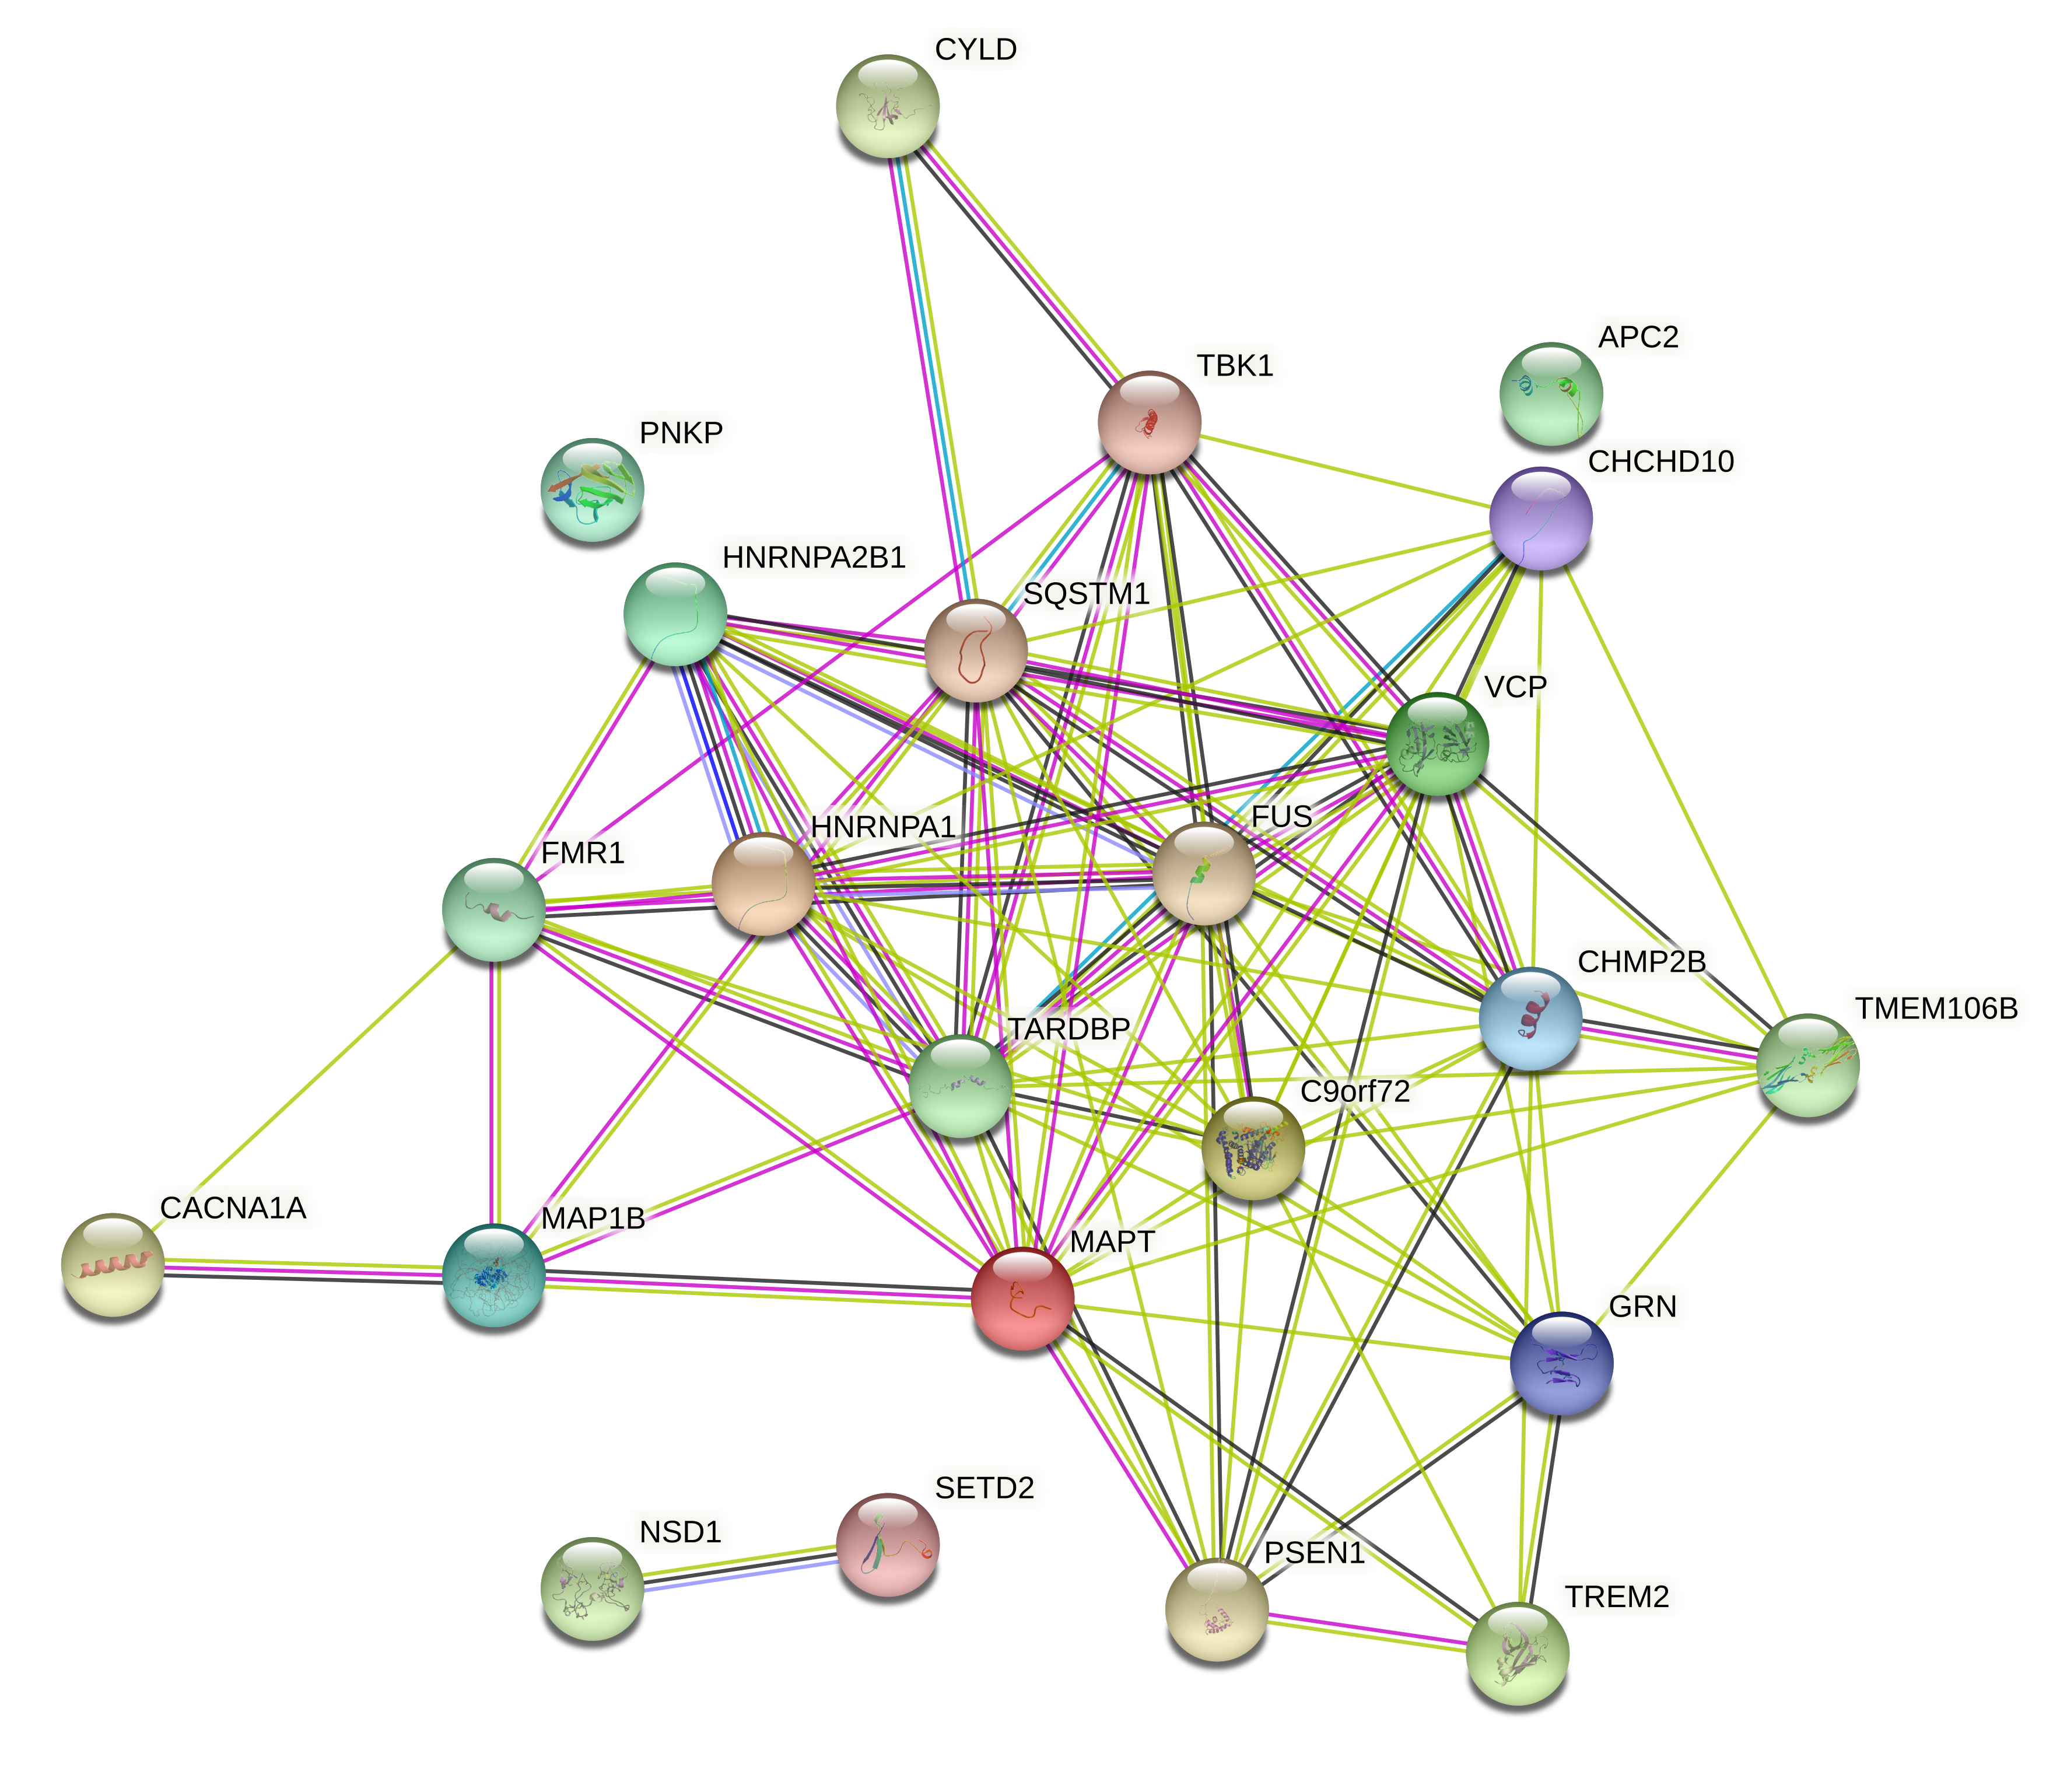
\includegraphics[width=0.90\textwidth]{figures/Gene_Relationship.png}
	\caption{Interacciones proteína-proteína a raíz de los genes relacionados. }
	\label{fig:string1}
\end{figure}

Una vez cargados los genes y sus relaciones en string, procedemos a descargar los ficheros "string-node-degree.tsv" e "string-interactions.tsv".

Se creara también un objeto network de la librería de R stringdb, con las siguientes caracteristicas:

Versión=11
Specie=9606
Score threshold=400

\hfill

Se usara esta network de genes humanos, para buscar genes vecinos de los 24 que teníamos en un principio y realizar una propagación de red con el fin de aumentar el total de genes a estudiar que guarden directa o indirectamente una relación con nuestro fenotipo a estudiar.

\hfill

\subsection{igraph}

Usaremos igraph para convertir nuestro objeto network (genes originalmente relacionados con el  fenotipo mas los genes vecinos de la red general anteriormente citada) en un dataframe que sea procesable por las funciones de clustering para la división en comunidades

\hfill

\subsection{Análisis por comunidades}

Se realizan a continuación los correspondientes pasos para clusterizar nuestro conjunto en distintas comunidades y realizar el correspondiente análisis de enriquecimiento funcional a las adecuadas:

\subsubsection{LinkComm}

Tras una serie de pruebas con distintas funciones de igraph para hacer comunidades, se ha decidido usar la anteriormente citada LinkComm, que nos deja esta imagen como muestra de su trabajo sobre nuestra red de genes: 

\begin{figure}[h]
	\centering
	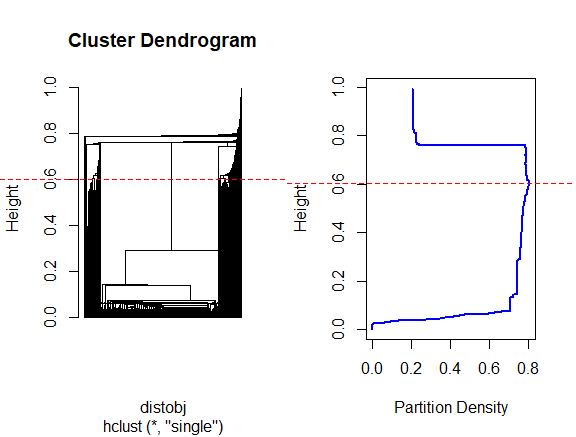
\includegraphics[width=0.90\textwidth]{figures/Grapichs_LinkComm.png}
	\caption{Dendograma del clustering realizado-Relación Altura con Densidad de particion. }
	\label{fig:string1}
\end{figure}

\hfill

\subsubsection{ClusterProfiler}

A continuación se realizara un enriquecimiento funcional con GO (Gene Ontology) para observar las funciones implicadas en la formación de las distintas componentes celulares de las comunidades con un número de genes similar a 20, que supone aproximadamente un 10/100 del total de nuestra red propagada. (En concreto las número 48,71 y 65 que tienen 24,22 y 19 genes respectivamente).

\hfill

Se muestran ahora las principales funciones obtenidas de los tres enriquecimientos:



\hfill
